\documentclass[runningheads]{llncs}
\usepackage[T1]{fontenc}
\usepackage{amsmath}

% define lightgray
\usepackage[table]{xcolor}

\usepackage{booktabs}
\usepackage[square,sort,comma,numbers]{natbib}
\usepackage[pdfstartview=XYZ,
bookmarks=true,
colorlinks=true,
linkcolor=blue,
urlcolor=blue,
citecolor=blue,
pdftex,
bookmarks=true,
linktocpage=true, % makes the page number as hyperlink in table of content
hyperindex=true
]{hyperref}

\usepackage{orcidlink} % orcidlink
\usepackage{marvosym} %letter symbol
\usepackage{rotating} % Rotating table
\usepackage{subcaption}
\usepackage{graphicx}

\title{Comparing efficiency, utility, and privacy between synthetic data packages and methods}
\titlerunning{Comparing efficiency, utility, and privacy}

\author{Jörg Drechsler\inst{1 (\text{\Letter})} \and
Jonathan Latner\inst{1 \orcidlink{0000-0002-1825-0097}} \and
Marcel Neunhoeffer\inst{1 \orcidlink{0000-0002-9137-5785}}}

% \author{Jörg Drechsler\inst{1} \and
% Jonathan Latner\inst{1,2}\url{http://orcid.org/0000-0002-9771-1276} \and
% Marcel Neunhoeffer\inst{1,3}\url{http://orcid.org/0000-0002-9137-5785}}

% \item \href{https://orcid.org/0000-0002-9771-1276}{\textcolor{orcidlogocol}{\aiOrcid} \hspace{2mm} orcid.org/0000-0002-9771-1276}

\authorrunning{Drechsler et al., \the\year}

\institute{Institute for Employment Research, Nuremberg, Germany
\email{{joerg.drechsler,jonathan.latner,marcel.neunhoeffer}@iab.de}}

\newcommand{\fix}{\marginpar{FIX}}
\newcommand{\new}{\marginpar{NEW}}

\begin{document}

\maketitle              % typeset the header of the contribution
%
\begin{abstract}
The abstract should briefly summarize the contents of the paper in
150--250 words.

\keywords{First keyword  \and Second keyword \and Another keyword.}
\end{abstract}


\clearpage

\section{Introduction}

% utility is task specific  - specific measures (cio)
% fidelity is how similar the data is to the original - broad/general measure (pmse)

The origins of releasing synthetic data instead of actual data are often understood to begin with Rubin \cite{rubin1993statistical}, who proposed a method for fully synthetic data, and Little \cite{little1993statistical}, who proposed a method for partially synthetic data.  Here, when we refer to data, we are referring to microdata (i.e. one observation per individual unit) as opposed to tabular data (i.e. summary data).  Releasing synthetic data means altering actual data in some way so that the released data do not contain information on a real individual unit (person, firm, etc.).  The advantage is more users can use data that would otherwise be not easily available.  The disadvantage is that the higher the level of privacy protection, the lower the level of `utility,' or the degree to which the real data match the synthetic data.  This is known as the privacy-utility or risk-accuracy trade-off \citep{reiter2010releasing}.  While a few recent papers evaluate synthetic data generators (SDGs), i.e. statistical packages that create synthetic data, on the trade-off between privacy and utility \citep{little2022comparing,dankar2021fake}, there is little discussion of the computational power, i.e. the duration in time or `efficiency' required to create synthetic data \citep{jordon2022synthetic}.  Efficiency is important because as the data being synthesized increase in dimensionality, the cost of releasing the data in human labour and computational time increases.  

We contribute to the literature not only by adding efficiency as a third dimension to the relationship between privacy and utility when evaluating SDGs, but by isolating the strength and weakness of different SDGs.  In this paper, we evaluate three common SDGs on the relationship between utility, privacy, and efficiency: Synthpop \cite{nowok2016synthpop}, CTGAN \cite{patki2016synthetic}, and DataSynthesizer \cite{ping2017datasynthesizer}.  Previous research also evaluated these SDGs \cite{dankar2021fake,little2022comparing}.  

One challenge to any evaluation of SDGs is that there is no agreement on how exactly to measure utility or privacy risk, let alone the relationship between the two.  We begin with utility measures.  There are two main types: broad and narrow measures \citep{drechsler2009disclosure}.  These are also sometimes known as global and analysis-specific measures \citep{woo2009global}.  Broad measures quantify some kind of statistical distance between original and synthetic data \citep{taub2020impact}.  In its simplest form, one can simply compare frequency counts between the same variable in the original and synthetic data.  However, not only does this only work in datasets with a limited number of variables, one-way frequency counts does not begin to capture the two- or three-way (or more) relationship to other variables.  As a result, other methods have been developed to capture these relationships, including Hellinger distance, Propensity Score Measure mean-squared error (pMSE), Kolmogorov-Smirnov statistic (KS), among many others.  Narrow measures compare parametric models or variables between original and synthetic data.  Examples include confidence-interval overlap (CIO) or ratio of estimates (ROE), either univariate or bivariate.  

A second challenge is that there is no agreement on what data should be used to evaluate these measures.  There are three main options.  One is publicly available data from a Census.  For example, Litte et al., \cite{little2022comparing} use Census from Canada, Fiji, Rwanda, and the United Kingdom.  A second option is to use publicly available data that are used in Machine Learning (ML) applications \citep{dankar2021fake}, from Kaggle, UC Irvine, Open ML, etc.  A third option is to use simulated data created.  Each option presents advantages and disadvantages, but there is little agreement on the role of three data components: dimensionality (number of rows and columns), missing observations, or correlated variables.  For example, while Census data are correlated, simulated data are often not.  On the other hand, simulated data are often high dimensional, but Census data are not.  Census data often include missing observations, but ML or simulated data often do not.  While simulated data can be as correlated as the user desires as well as include missing values, and Census data can be highly dimensional, the choice of what data should be used to evaluate is a subjective research choice that will indicate the strength or weakness of a given SDG, even if a different data set could suggest the opposing conclusion.

A third challenge is that there is a difference between a statistical package that creates synthetic data and the method they use.  One should not confuse the two.  For example, Generative Adversarial Networks (GANs) are gaining increasing attention as SDG, but there are not only many different types of GANs, there are also many types of SDGs that use GANs.  Therefore, the advantages or disadvantages of one GAN relative to other SDGs is not necessarily a reflection of all GANs.  Similarly, a popular package for the creation of synthetic data is called Synthpop in R that relies on Classification and Regression Trees (CART) models \citep{nowok2016synthpop}.  However, there is no one type of CART model.  For example, the MICE package in R also uses a CART model \citep{van2011mice}.  Further, while the Synthpop package implements the CART model described by Reiter \cite{reiter2005using}, this is not the same thing as the general description of SDG described by Rubin \cite{rubin1993statistical}.  The point is that one needs to distinguish between a method and a package when evaluating SDG tools.

The evidence presented here adds considerable nuance to our understanding of SDGs.  We not only find that Synthpop provides the highest levels of utility with the lowest levels of risk (replicating previous research), we also find that Synthpop is a highly efficient SDG with respect to the time required to create a synthetic data set.  However, this finding is conditional on low-dimensional data.  In the event of data with at least one categorical variable containing at least 25 values, the advantage with respect to efficiency.  What was once a $~$40x advantage in speed, becomes a $~$10x disadvantage.  This problem is exacerbated as one increases the dimensionality, especially with respect to columns.  While Synthpop retains its superiority with respect to the risk-accuracy trade-off, other SDGs that may not have been considered to be comparable, become viable.  Without denying the obvious appeal or strengths of Synthpop, we isolate its weakness and, in so doing, illustrate the comparable strengths of other SDGs.

\section{Background}

There is a link between the methods and goals for releasing synthetic data.  After all, methods that are designed to achieve one goal may not be well-suited to achieve a different goal.  In the beginning, there were two main approaches that were developed in parallel, but were also disconnected from one another \citep{drechsler202330}: the statistical approach and the computer science approach.  

\subsection{Statistical approaches}

As described by Rubin \cite{rubin1993statistical}, the original idea was that if a statistical agency could generate synthetic microdata sets for public use, none of which was an observed unit in the actual data, then this would achieve multiple goals.  For the survey participants, they could be confident that confidential data would never be released, which would increase the likelihood not only of more survey respondents, but also more truthful answers.  For the illegitimate user or `snooper,' the value of the data would be eliminated because they could not discover actual, confidential information.  Finally, for the legitimate user, the value of the data would increase not only because the data are easier to access, but also more accurate than the actual data.\footnote{``Experience with these data sets shows that inferences for population estimands involving $Y$ based on the multiply-imputed public-use file appear to be valid, and often, perhaps even typically, $more$ precise [emphasis in original] than the corresponding inferences based on the research file, despite the fact that only entirely synthetic $Y$ vvalues exist in the public-use file and all the real $Y$ values exist in the research file \citep[pg. 466]{rubin1993statistical}.''}  

To create synthetic data from actual data, all non-respondents in a survey are treated as missing values to be replaced with `imputed' values.  Given a dataset ($D$) with observations ($n$), there is a two-stage process.  First, a model for predicting a given outcome variable ($y$) given a set of background variables ($x$) is trained on the actual data.  Second, values of the original outcome variable are replaced by predicted values of the outcome variable ($y^*$).  This process is then repeated so that all actual values are replaced by imputed values for every variable.  The result is a multiply-imputed synthetic dataset ($D^*$) that contains no values in the actual data, but looks structurally identical to the actual data, not only with respect to mean and variation of a given variable, but also correlations between variables.  As a final step, one can release multiple samples of the synthetic data ($M$), each of which contain a random draw of individuals from the synthetic dataset ($D^*$) in order to ensure that the samples exclude actual units that are generated by the two-stage process.

Despite the advantages of the method, implementing the two-stage process is more complicated than the simple description might suggest.  The importance of model selection in the first stage cannot be understated.  There are two central problems or questions.  The first problem is the question of what is the first variable to be imputed.  Given that different data contain different variables, it is not possible to create a uniform or general rule that is objectively agreed to be correct.  While the decision remains a subjective research choice, common guidelines are understood and agreed upon (XXXX).  For example, it is preferable for the first outcome variable to be a continuous variable, or at minimum not a dichotomous variable.  Of course, this may not always be possible in every dataset.  

The second problem is the question of what model to use.  While Rubin may have had in mind some sort of parametric estimation using a linear or non-linear model, there is now general agreement that Classification and Regression Trees (CART) models provide the highest level of utility \citep{drechsler2011empirical}.  However, even if it is agreed that CART models are the standard (which it is not), two new problems are created.  First, there is no one, single CART model.  Different synthetic data generators (SDGs) may implement their own variation or flavour.  Second, and related, there may not necessarily be a match between an empirical implementation of CART and its theoretical implementation described by Rubin.  We return to this issue in the methods section.

While the statistical approach addresses both utility and privacy, the methodological emphasis is on utility.  Privacy is achieved by the SDG in the second stage, where no actual data are in the synthetic data.  The obvious problem is that with a sufficiently accurate model, one with high levels of utility, the model itself could reproduce actual data in the synthetic data.  Rubin \cite{rubin1993statistical} acknowledged this possibility, and suggested to draw samples ($M$) after excluding actual, reproduced units.  However, the more general critique is that the statistical approach offers no formal guarantee for privacy protection or measure of privacy risk.  This leads directly to the computer science approach to synthetic data.

\subsection{Computer science approaches}

In the computer science approach, the original idea was to measure privacy risk, not methods for producing synthetic data.  Examples include: k-anonymity \citep{sweeney2002k}, l-diversity \citep{machanavajjhala2007diversity}, or t-closeness \citep{li2006t}.  We do not mean to suggest that the statistical approach is not interested in privacy risk.  To the contrary, reducing privacy risk is one of the main goals of releasing synthetic data.  At the same time, we do not mean to suggest that the computer science approach is not interested in utility.  The difference is that in that in the statistical approach, privacy risk was not measured, but rather built into the process of releasing samples that contain no actual units.  By contrast, in the computer science approach, measuring privacy risk is central.  It was not until the concept of differential privacy (DP) \citep{dwork2006calibrating} was developed that computer scientists began to develop applications and methods to create synthetic data.  

Differential privacy is a theoretical concept, but the basic idea is the it measures the degree to which \dots


\subsection{Other advantages of synthetic data}

Another advantage of publicly available synthetic data can help users develop code so that when they gain access to the actual data, they may use their time more efficiently.  Under these conditions, one may imagine that standards for utility decline, even if standards for privacy are maintained, but that is not correct.  If utility declines too much, then the resulting code may not be applicable when using the actual data.  {\bf JPL note: Is there a good example or citation for this?}

\section{Research design}

Our goal is to compare and contrast synthetic data generators (SDGs) on the degree to which the provide high levels of utility, low levels of privacy risk, and are computationally efficient in terms of the duration required to create a synthetic dataset.  While previous research has done this \citep{little2022comparing,dankar2021fake}, flaws exist in their research design with respect to the data, risk/utility measures, and the importance of tuning.  

\subsection{Synthetic data generators (SDGs)}


There is a link between the statistical packages that contain synthetic data generators (SDGs) and the methods they use, but the link is not exact and one should not assume that a package is the same as the method or visa versa.

\subsubsection{Classification and Regression Trees (CART)}

To illustrate the challenge, we use the Synthpop package in R \citep{nowok2016synthpop}.  While Synthpop generates synthetic data from both parametric and nonparametric models, the CART model is the default.  According to the online description,\footnote{\url{https://www.synthpop.org.uk/about-synthpop.html\#methodology}} Synthpop follows the two-stage process described by Rubin \citep{rubin1993statistical}.  However, if one actually looks at the code,\footnote{https://github.com/cran/synthpop/blob/master/R/functions.syn.r} there is an important difference.  Instead of replacing $y$ with $y^*$ generated by the model, Synthpop replaces $y$ with the leaf number from the regression tree (line 523-523).  Then, Synthpop predicts the leaf number (line 527) for $y$.  Finally, Synthpop replaces the predicted leaf number with sampled values of $y$ from the actual data in that leaf (line 549).  The point: the second-stage replaces values in the synthetic data ($D^*)$ with values in the actual data ($D$).  

We are not suggesting that we are revealing some sort of hidden secret.  Even if many users may not be aware, not only is the implementation used in Synthpop based on Reiter \cite{reiter2005using}, it is also well documented in the code with comments.\footnote{We do note that the code does not necessarily match with the methodological description, which more generally follows Rubin \cite{rubin1993statistical}.}  However, we also believe that one reason why Synthpop has such high levels of utility is because the SDG used in Synthpop samples from the actual data and, related, this implementation does not strictly follow Rubin \cite{rubin1993statistical}.   Therefore, our point is that Synthpop will by definition produce synthetic data sets with higher levels of utility than SDGs that more strictly follow Rubin and only sample from predicted values.  

Despite our critique, we must also ask, should users care?  If Synthpop produces higher levels of utility and higher levels of privacy protection using available metrics, then maybe the problem lies not with Synthpop, but rather a strict implementation of Rubin's description.  At the same time, as we will describe in more details later, it is difficult to know for sure if Synthpop produces higher levels of utility and privacy because there is no one agreed upon measure.  Given that, perhaps it is better to separate the actual data from the data generator if for no other reason than it is simply how it should be done.  At this point, we remain agnostic, but it is an issue we return to throughout this article.

More generally, Synthpop is not CART and CART is not Synthpop.  As we have described, Synthpop implements a variation of the CART package.  It is a defensible research choice, but other SDGs may implement their own variation of CART that is also defensible.  For example, the MICE package in R also uses a CART model \citep{van2011mice}, which can also be used to generate synthetic data \citep{volker2021anony}.  

\subsubsection{General adversarial networks (GANs)}

More recently, Generative Adversarial Networks (GANs) have become popular.  In the original application, GANs reproduced photographic images of numbers, human faces, and animals \citep{goodfellow2014generative}.  To understand what GANs do, we begin with supervised machine learning (ML) models that are used to generate a prediction.  ML models use training data as input that are then used by the model to generate a predicted output.  Model fit is determined by comparing the predicted output with the actual output in the training data.  Based on the degree of model fit, users can update the model.  

GANs are a form of unsupervised ML models, sometimes referred to as deep learning (DL) models.  In a GAN, there are two submodels, a generator and a discriminator.  A generators creates fake input and a discriminators decides if the input from the generator is fake from the generator or real from the training data.  The relationship between the two models are `adversarial.'  As the discriminator rejects input from the generator as fake, the generator updates the model to become more and more accurate.  Eventually, the discriminator cannot determine if the generated input is fake or real.  In the original application, a discriminator may not have been able to distinguish between an actual from a fake image of a number \citep{goodfellow2014generative}, but a human could.  Over time, output from GANs have become harder for humans to distinguish (XXXX).

While not intended to create synthetic data, it is easy to see why GANs could be appealing.  If a GAN could successfully reproduce an image to the point that a human could not distinguish a real image from a fake one, then its seems logical to assume that a GAN could successfully reproduce tabular data with such high levels of utility that a user could not distinguish whether the underlying data were actual or synthetic.  Like Synthpop, GANs offer no formal guarantee for privacy, despite the fact that GANs come from the computer science literature.  Instead, like Synthpop, privacy is derived from the fact that the discriminator acts like the second stage in Rubin's process and never touches the actual data.  In reality, one can adjust the training procedure of the discriminator to satisfy a formal guarantee \citep{beaulieu2019privacy,neunhoeffer2020private}.

We raise two concerns about GANs: not only are they poor SDGs in terms of utility (XXXX), but they are also computationally intensive in the sense that they may take hours, days, or even weeks to train.  For these reasons, one may assume that GANs are an inferior SDG compared to Synthpop, but that may not be correct.  Here, we must distinguish GANs the method from statistical packages that implement them.  GANs come in many flavours and a GAN that is well suited to reproduce an image may not be well suited to reproduce tabular data.  The question is: Can we build a better GAN?  As we will show, the answer is yes we can.  The second concern is with respect to the computational power and time required to train a GAN.  While Synthpop is more efficient in low-dimensional data, GANs are more efficient in high-dimensional data.  As we will show, common conditions exist where GANs are faster than Synthpop.

\subsubsection{Bayesian Networks}

Bayesian methods build directly on the concept of differential privacy (DP), as originated in the computer science approach.  The appeal is objective.  Between 2018 and 2019, the National Institute of Standards and Technology (NIST) held three rounds of the Differential Privacy Synthetic Data Challenge (Challenge.gov, 2019).  The winning teams relied on Bayesian networks or approaches to preserve pre-specified marginal distributions.  Datasynthesizer is a Python package that implements PrivBayes \citep{zhang2017privbayes}.  Datasynthesizer is the only package that includes a parameter that users may set to control for differential privacy ($\epsilon$).  

While the default is 0.1, 0 is off, there is no theoretical top end.

\subsection{Data}

The choice of what type of data to use to compare and contrast SDGs is essential.  As mented earlier, the reason is that SDGs were designed for distinct types of data.  Synthpop was designed for Census data, GANs were designed for images, and PrivBayes was designed for relational databases.

Given that SDGs were designed for distinct types of data, it is hard to find a dataset that would 

\subsection{Evaluating utility}

\subsection{Evaluating privacy}

\subsubsection*{Acknowledgments}
Use unnumbered third level headings for the acknowledgments. All acknowledgments, including those to funding agencies, go at the end of the paper. Only add this information once your submission is accepted and deanonymized. 

\clearpage
\bibliographystyle{splncs04}
\bibliography{references}

%%%%%%%%%%%%%%%%%%%%%%%%%%%%%%%%
% Tables
%%%%%%%%%%%%%%%%%%%%%%%%%%%%%%%%

\clearpage
\section{Tables}

\vskip -5mm
\begin{table}[!htb]
\minipage{\textwidth}
% \begin{table}
    \caption{Social Diagnosis 2011 (SD2011)}
    \centering
    \rowcolors{1}{white}{lightgray}
    \resizebox{\textwidth}{!}{% latex table generated in R 4.4.0 by xtable 1.8-4 package
% Thu Sep 26 09:11:53 2024
\begin{tabular}{rlllllllll}
  \toprule
Number & Variable & Description & Type & Observations & Unique.Values & Missings & Negative.values & Generated & Messy \\ 
  \midrule
  1 & sex & Sex & factor & 5000 & 2 & 0 & 0 &  &  \\ 
    2 & age & Age of person, 2011 & numeric & 5000 & 79 & 0 & 0 &  &  \\ 
    3 & agegr & Age group, 2011 & factor & 5000 & 7 & 4 & 0 & Yes & Yes \\ 
    4 & placesize & Category of the place of residence & factor & 5000 & 6 & 0 & 0 &  &  \\ 
    5 & region & Region (voivodeship) & factor & 5000 & 16 & 0 & 0 &  &  \\ 
    6 & edu & Highest educational qualification, 2011 & factor & 5000 & 5 & 7 & 0 &  &  \\ 
    7 & eduspec & Discipline of completed qualification & factor & 5000 & 28 & 20 & 0 &  &  \\ 
    8 & socprof & Socio-economic status, 2011 & factor & 5000 & 10 & 33 & 0 &  &  \\ 
    9 & unempdur & Total duration of unemployment in the last 2 years (in months) & numeric & 5000 & 30 & 0 & 1556 &  &  \\ 
   10 & income & Personal monthly net income & numeric & 5000 & 407 & 683 & 603 &  & Yes \\ 
   11 & marital & Marital status & factor & 5000 & 7 & 9 & 0 &  &  \\ 
   12 & mmarr & Month of marriage & numeric & 5000 & 13 & 1350 & 0 &  &  \\ 
   13 & ymarr & Year of marriage & numeric & 5000 & 75 & 1320 & 0 &  &  \\ 
   14 & msepdiv & Month of separation/divorce & numeric & 5000 & 13 & 4300 & 0 &  &  \\ 
   15 & ysepdiv & Year of separation/divorce & numeric & 5000 & 51 & 4275 & 0 &  &  \\ 
   16 & ls & Perception of life as a whole & factor & 5000 & 8 & 8 & 0 &  &  \\ 
   17 & depress & Depression symptoms indicator & numeric & 5000 & 23 & 89 & 0 &  &  \\ 
   18 & trust & View on interpersonal trust & factor & 5000 & 4 & 37 & 0 &  &  \\ 
   19 & trustfam & Trust in own family members & factor & 5000 & 4 & 11 & 0 &  &  \\ 
   20 & trustneigh & Trust in neighbours & factor & 5000 & 4 & 11 & 0 &  &  \\ 
   21 & sport & Active engagement in some form of sport or exercise & factor & 5000 & 3 & 41 & 0 &  &  \\ 
   22 & nofriend & Number of friends & numeric & 5000 & 44 & 0 & 41 &  & Yes \\ 
   23 & smoke & Smoking cigarettes & factor & 5000 & 3 & 10 & 0 &  &  \\ 
   24 & nociga & Number of cigarettes smoked per day & numeric & 5000 & 30 & 0 & 3737 &  & Yes \\ 
   25 & alcabuse & Drinking too much alcohol & factor & 5000 & 3 & 7 & 0 &  &  \\ 
   26 & alcsol & Starting to use alcohol to cope with troubles & factor & 5000 & 3 & 82 & 0 &  &  \\ 
   27 & workab & Working abroad in 2007-2011 (in months) & factor & 5000 & 3 & 438 & 0 &  &  \\ 
   28 & wkabdur & Total time spent on working abroad & numeric & 5000 & 33 & 0 & 4875 &  & Yes \\ 
   29 & wkabint & Plans to go abroad to work in the next two years & factor & 5000 & 4 & 36 & 0 &  &  \\ 
   30 & wkabintdur & Intended duration of working abroad & factor & 5000 & 6 & 4697 & 0 &  &  \\ 
   31 & emcc & Intended destination country & factor & 5000 & 18 & 4714 & 0 &  &  \\ 
   32 & englang & Knowledge of English language & factor & 5000 & 4 & 15 & 0 &  &  \\ 
   33 & height & Height of person & numeric & 5000 & 65 & 35 & 0 &  &  \\ 
   34 & weight & Weight of person & numeric & 5000 & 91 & 53 & 0 &  &  \\ 
   35 & bmi & Body mass index (weight - kg/(height - cm$^2$)*10000) & numeric & 5000 & 1396 & 59 & 0 & Yes & Yes \\ 
   \bottomrule
\end{tabular}
}
    % % latex table generated in R 4.4.0 by xtable 1.8-4 package
% Thu Sep 26 09:11:53 2024
\begin{tabular}{rlllllllll}
  \toprule
Number & Variable & Description & Type & Observations & Unique.Values & Missings & Negative.values & Generated & Messy \\ 
  \midrule
  1 & sex & Sex & factor & 5000 & 2 & 0 & 0 &  &  \\ 
    2 & age & Age of person, 2011 & numeric & 5000 & 79 & 0 & 0 &  &  \\ 
    3 & agegr & Age group, 2011 & factor & 5000 & 7 & 4 & 0 & Yes & Yes \\ 
    4 & placesize & Category of the place of residence & factor & 5000 & 6 & 0 & 0 &  &  \\ 
    5 & region & Region (voivodeship) & factor & 5000 & 16 & 0 & 0 &  &  \\ 
    6 & edu & Highest educational qualification, 2011 & factor & 5000 & 5 & 7 & 0 &  &  \\ 
    7 & eduspec & Discipline of completed qualification & factor & 5000 & 28 & 20 & 0 &  &  \\ 
    8 & socprof & Socio-economic status, 2011 & factor & 5000 & 10 & 33 & 0 &  &  \\ 
    9 & unempdur & Total duration of unemployment in the last 2 years (in months) & numeric & 5000 & 30 & 0 & 1556 &  &  \\ 
   10 & income & Personal monthly net income & numeric & 5000 & 407 & 683 & 603 &  & Yes \\ 
   11 & marital & Marital status & factor & 5000 & 7 & 9 & 0 &  &  \\ 
   12 & mmarr & Month of marriage & numeric & 5000 & 13 & 1350 & 0 &  &  \\ 
   13 & ymarr & Year of marriage & numeric & 5000 & 75 & 1320 & 0 &  &  \\ 
   14 & msepdiv & Month of separation/divorce & numeric & 5000 & 13 & 4300 & 0 &  &  \\ 
   15 & ysepdiv & Year of separation/divorce & numeric & 5000 & 51 & 4275 & 0 &  &  \\ 
   16 & ls & Perception of life as a whole & factor & 5000 & 8 & 8 & 0 &  &  \\ 
   17 & depress & Depression symptoms indicator & numeric & 5000 & 23 & 89 & 0 &  &  \\ 
   18 & trust & View on interpersonal trust & factor & 5000 & 4 & 37 & 0 &  &  \\ 
   19 & trustfam & Trust in own family members & factor & 5000 & 4 & 11 & 0 &  &  \\ 
   20 & trustneigh & Trust in neighbours & factor & 5000 & 4 & 11 & 0 &  &  \\ 
   21 & sport & Active engagement in some form of sport or exercise & factor & 5000 & 3 & 41 & 0 &  &  \\ 
   22 & nofriend & Number of friends & numeric & 5000 & 44 & 0 & 41 &  & Yes \\ 
   23 & smoke & Smoking cigarettes & factor & 5000 & 3 & 10 & 0 &  &  \\ 
   24 & nociga & Number of cigarettes smoked per day & numeric & 5000 & 30 & 0 & 3737 &  & Yes \\ 
   25 & alcabuse & Drinking too much alcohol & factor & 5000 & 3 & 7 & 0 &  &  \\ 
   26 & alcsol & Starting to use alcohol to cope with troubles & factor & 5000 & 3 & 82 & 0 &  &  \\ 
   27 & workab & Working abroad in 2007-2011 (in months) & factor & 5000 & 3 & 438 & 0 &  &  \\ 
   28 & wkabdur & Total time spent on working abroad & numeric & 5000 & 33 & 0 & 4875 &  & Yes \\ 
   29 & wkabint & Plans to go abroad to work in the next two years & factor & 5000 & 4 & 36 & 0 &  &  \\ 
   30 & wkabintdur & Intended duration of working abroad & factor & 5000 & 6 & 4697 & 0 &  &  \\ 
   31 & emcc & Intended destination country & factor & 5000 & 18 & 4714 & 0 &  &  \\ 
   32 & englang & Knowledge of English language & factor & 5000 & 4 & 15 & 0 &  &  \\ 
   33 & height & Height of person & numeric & 5000 & 65 & 35 & 0 &  &  \\ 
   34 & weight & Weight of person & numeric & 5000 & 91 & 53 & 0 &  &  \\ 
   35 & bmi & Body mass index (weight - kg/(height - cm$^2$)*10000) & numeric & 5000 & 1396 & 59 & 0 & Yes & Yes \\ 
   \bottomrule
\end{tabular}

    \label{table:sd2011_data_structure}
% \end{table}
\endminipage

\vskip 5mm
\minipage{\textwidth}
% \begin{table}
    \caption{Ratio of estimates (ROE)}
    \centering
    \rowcolors{1}{white}{lightgray}
    \resizebox{.5\textwidth}{!}{% latex table generated in R 4.3.2 by xtable 1.8-4 package
% Wed May  1 12:47:00 2024
\begin{tabular}{lrrr}
  \toprule
variable & ctgan & datasynthesizer & synthpop \\ 
  \midrule
BMI & 0.21 & 0.21 & 0.24 \\ 
  Education & 0.88 & 0.99 & 0.94 \\ 
  Number of friends & 0.28 & 0.17 & 0.40 \\ 
  Work abroad duration & 0.06 & 0.29 & 0.38 \\ 
   \bottomrule
\end{tabular}
}
    \label{table:table_compare_roe}
% \end{table}
\endminipage

\vskip 5mm
\minipage{\textwidth}
% \begin{table}
    \centering
    \caption{Duration (in seconds)}
    \rowcolors{1}{white}{lightgray}
    \resizebox{\textwidth}{!}{% latex table generated in R 4.4.0 by xtable 1.8-4 package
% Fri Jul 19 16:14:31 2024
\begin{tabular}{llrrrr}
  \toprule
version & description & ctgan & datasynthesizer & synthpop (csv) & synthpop (package) \\ 
  \midrule
v00 & Raw (SD2011) & 331.01 & 245.37 & 2132.12 & 5474.39 \\ 
  v01 & Without eduspec or wkabdur & 290.30 & 264.43 & 10.99 & 8.45 \\ 
  v02 & Without wkabdur & 337.07 & 351.76 & 13.96 & 11.02 \\ 
  v03 & Without eduspec & 306.46 & 351.24 & 11.39 & 8.92 \\ 
  v04 & Last variables: eduspec-wkabdur & 374.57 & 344.02 & 14.23 & 287.85 \\ 
  v05 & Last variables: wkabdur-eduspec & 419.60 & 339.92 & 14.60 & 3657.55 \\ 
  v06 & as.numeric(wkabdur) and last variable: eduspec & 356.02 & 347.36 & 14.12 & 11.05 \\ 
  v07\_1\_20 & + 1 factor variable (20 values) & 339.05 & 264.96 & 42.23 &  \\ 
  v07\_1\_25 & + 1 factor variable (25 values) & 400.28 & 326.84 & 137.47 &  \\ 
  v07\_1\_30 & + 1 factor variable (30 values) & 339.73 & 269.72 & 363.18 &  \\ 
  v07\_2\_20 & + 2 factor variable (20 values) & 369.74 & 339.45 & 74.96 &  \\ 
  v07\_2\_25 & + 2 factor variable (25 values) & 364.56 & 361.81 & 631.43 &  \\ 
  v07\_2\_30 & + 2 factor variable (30 values) & 373.25 & 346.15 & 1222.54 &  \\ 
  v07\_3\_20 & + 3 factor variable (20 values) & 393.99 & 369.58 & 122.77 &  \\ 
  v07\_3\_25 & + 3 factor variable (25 values) & 401.03 & 383.40 & 881.53 &  \\ 
  v07\_3\_30 & + 3 factor variable (30 values) & 394.44 & 424.64 & 3654.59 &  \\ 
   \bottomrule
\end{tabular}
}
    \label{table:table_sd2011_duration}
    \\
    \raggedright
    \tiny{Notes: Synthpop (csv) indicates that SD2011 was loaded into R from a csv file.  Synthpop (package) indicates that SD2011 was loaded into R from the Synthpop package.}
% \end{table}
\endminipage
\end{table}

%%%%%%%%%%%%%%%%%%%%%%%%%%%%%%%%
% Graphs
%%%%%%%%%%%%%%%%%%%%%%%%%%%%%%%%

\clearpage
%%%%%%%%%%%%%%%%%%%%%%%%%%%%%%%%%%%%%%
% Graphs
%%%%%%%%%%%%%%%%%%%%%%%%%%%%%%%%%%%%%%
\clearpage
\section{Graphs}

\begin{figure}[ht]
    \caption{Comparing Synthetic Data Generators (pMSE)}
    \label{fig:graph_fidelity_compare}
    \centering

    \begin{subfigure}{\textwidth}
        \caption{pMSE}
        \resizebox{\textwidth}{!}{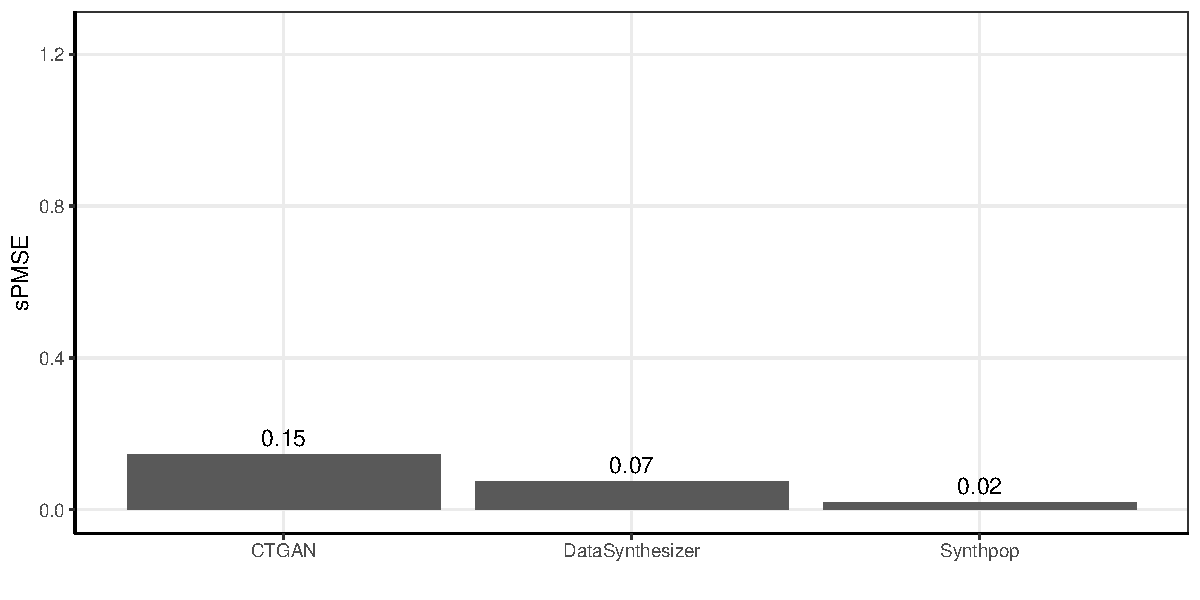
\includegraphics{../graphs/graph_fidelity_compare_dataset.pdf}}
        \label{subfig:graph_fidelity_compare_dataset}
    \end{subfigure}

    \begin{subfigure}{\textwidth}
        \caption{Two-way pMSE}
        \resizebox{\textwidth}{!}{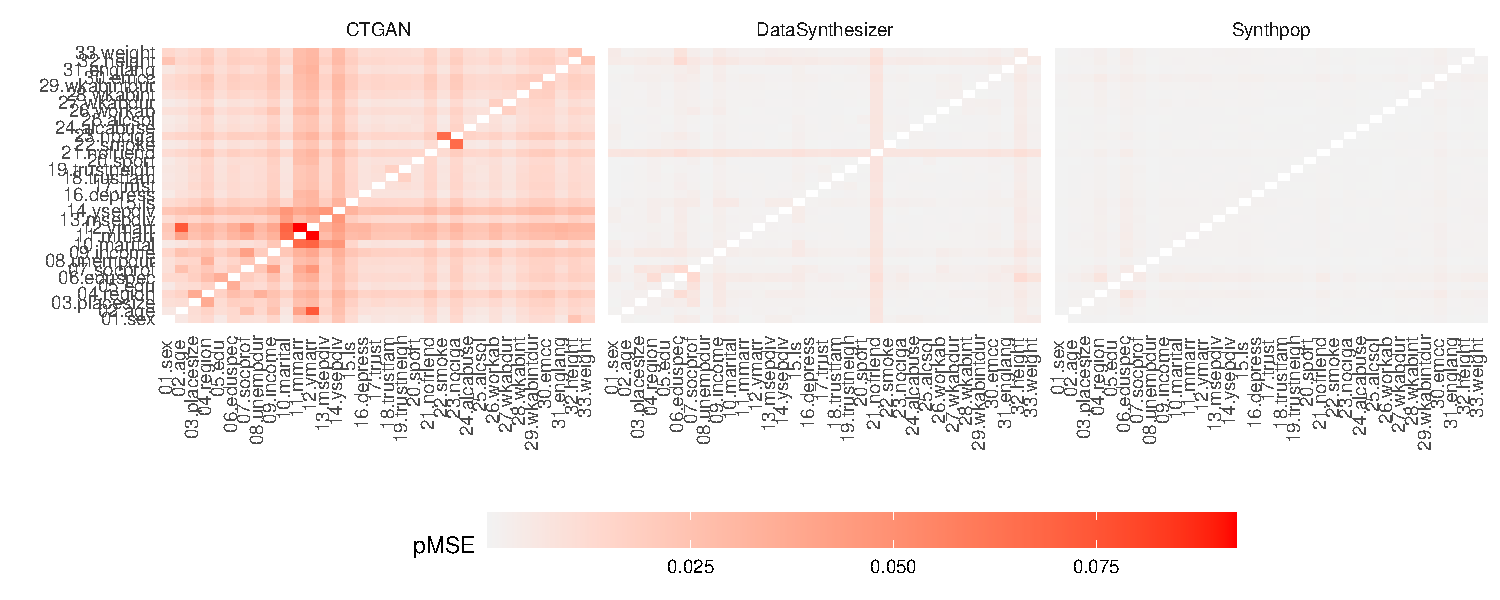
\includegraphics{../graphs/graph_fidelity_twoway_compare.pdf}}
        \label{subfig:graph_fidelity_compare_twoway}
    \end{subfigure}
\end{figure}


\begin{figure}[ht]
    \caption{Comparing one-way frequency of select variables and ROE}
    \label{fig:graph_frequency_compare}
    \centering

    \begin{subfigure}{\textwidth}
        \centering        
        \caption{Number of friends}
        \resizebox{.9\textwidth}{!}{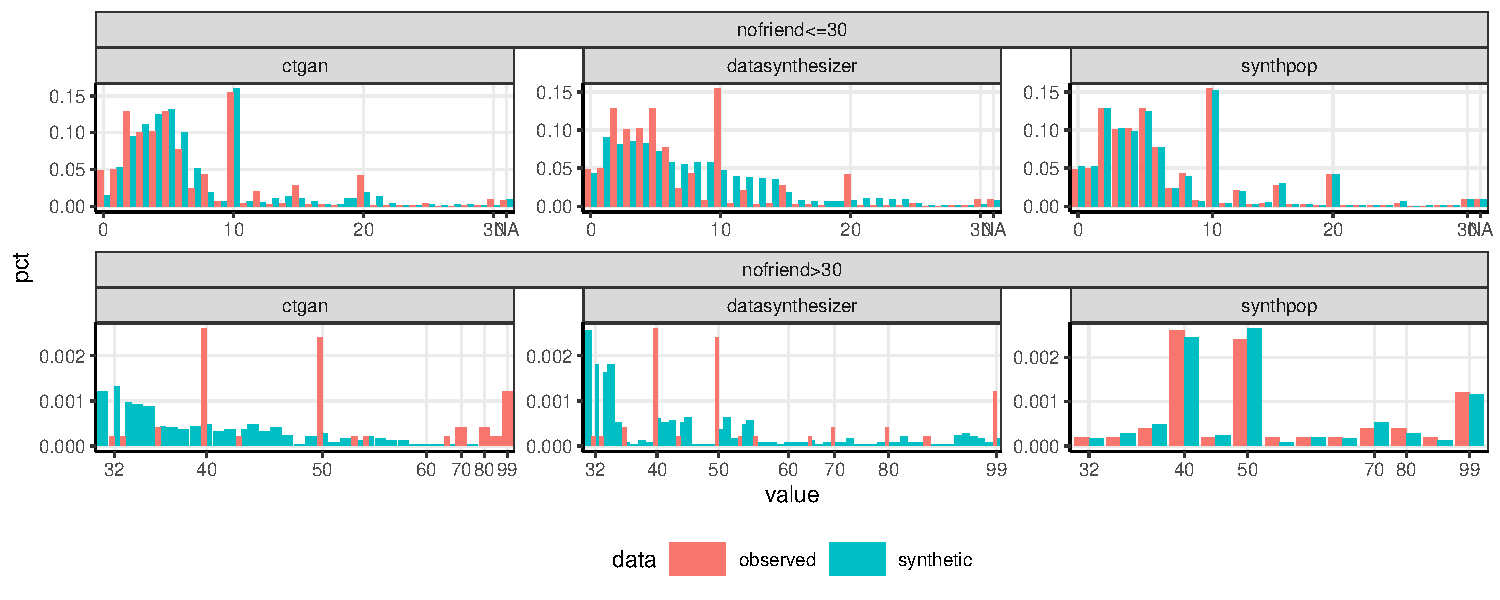
\includegraphics{../graphs/compare_nofriend_1.pdf}}
        \label{subfig:graph_frequency_compare_nofriend}
    \end{subfigure}

    \begin{subfigure}{\textwidth}
        \centering        
        \caption{BMI}
        \resizebox{.9\textwidth}{!}{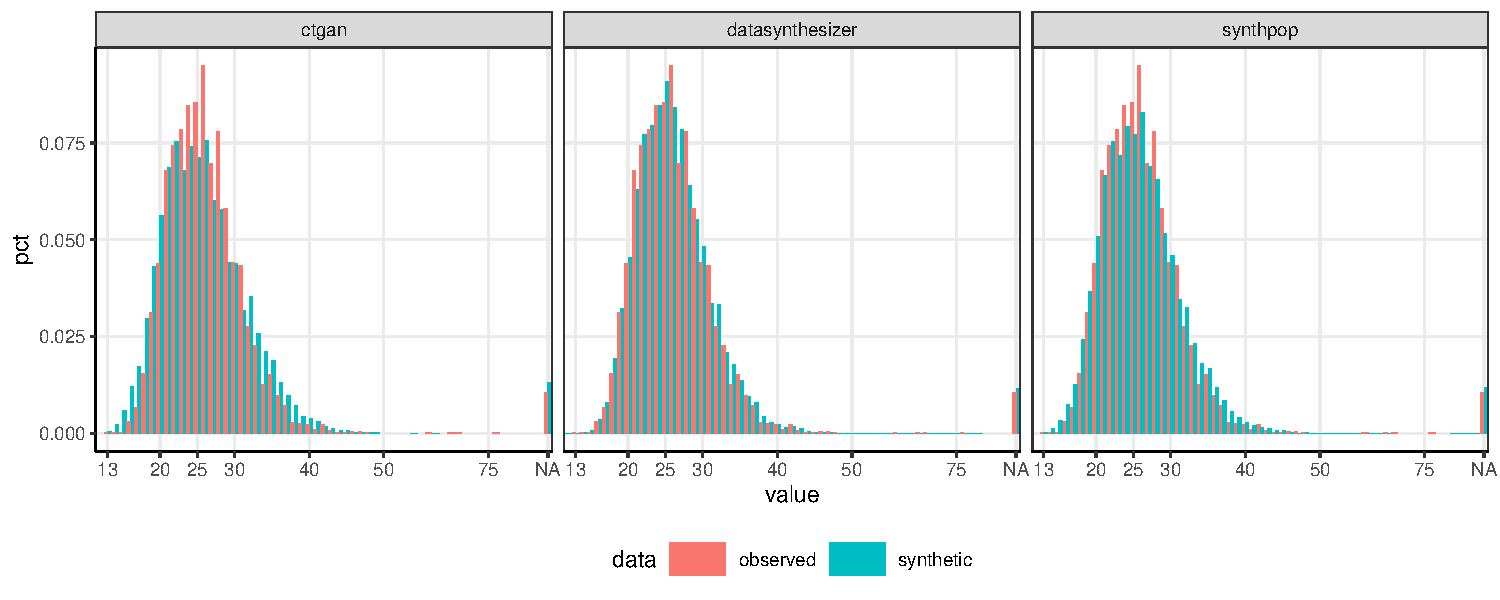
\includegraphics{../graphs/compare_bmi_1.pdf}}
        \label{subfig:graph_frequency_compare_bmi}
    \end{subfigure}

    \begin{subfigure}{\textwidth}
        \centering        
        \caption{Work abroad duration}
        \resizebox{.9\textwidth}{!}{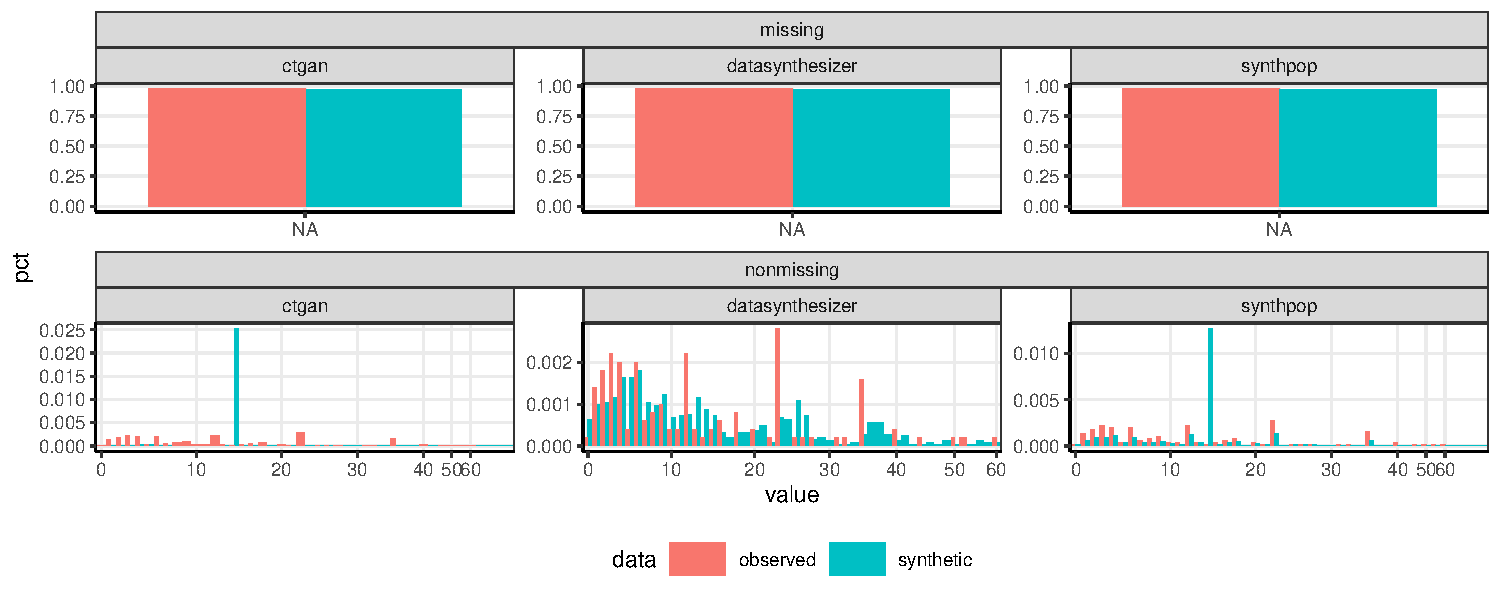
\includegraphics{../graphs/compare_wkabdur_1.pdf}}
        \label{subfig:graph_frequency_compare_wkabdur}
    \end{subfigure}

    \begin{subfigure}{\textwidth}
        \centering        
        \caption{Ratio of estimates (ROE)}
        \resizebox{.9\textwidth}{!}{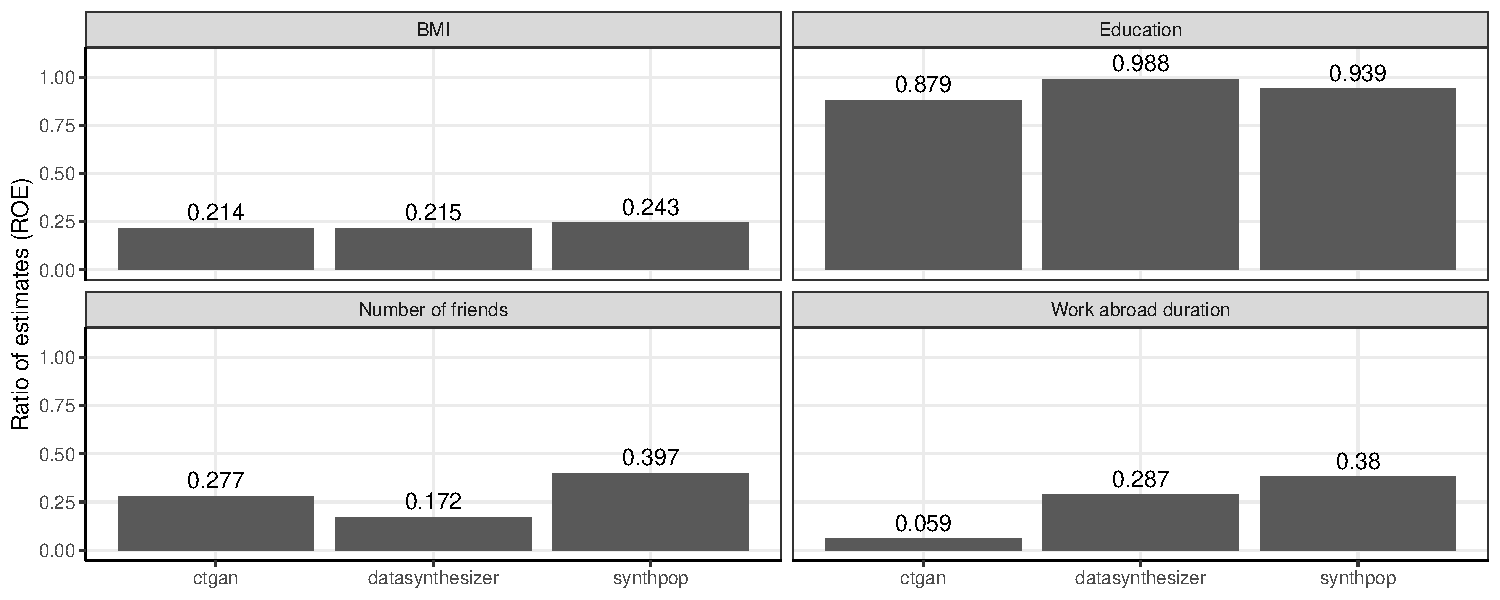
\includegraphics{../graphs/graph_compare_roe.pdf}}
        \label{subfig:graph_compare_roe}
    \end{subfigure}
\end{figure}

\begin{figure}
    \caption{Confidence interval overlap}
    \resizebox{\textwidth}{!}{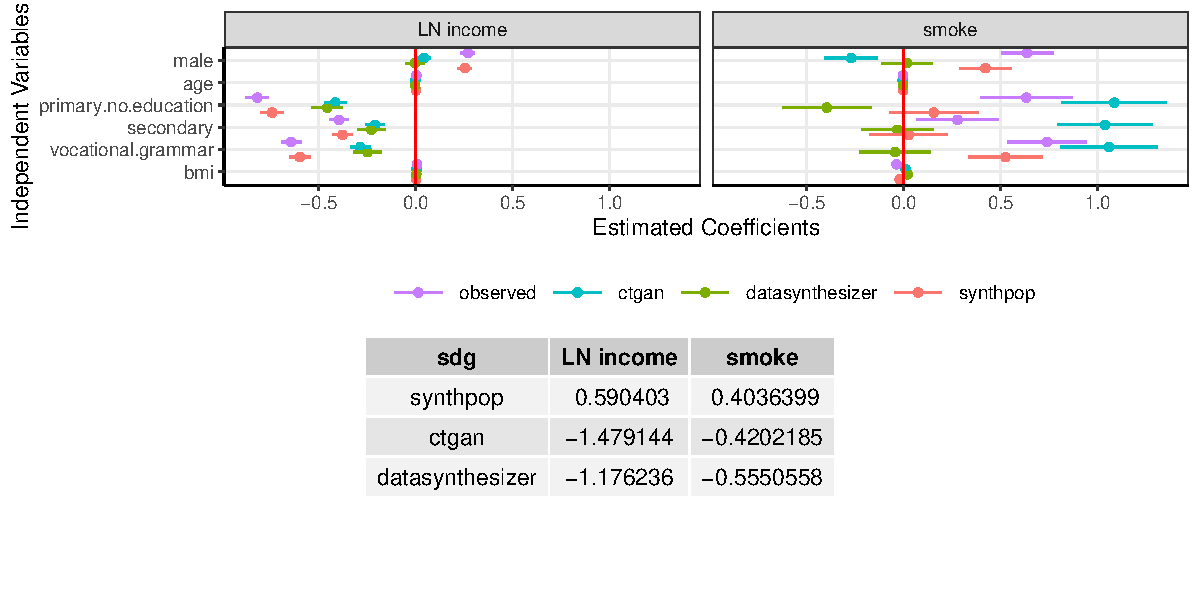
\includegraphics{../graphs/graph_utility_regression_cio_both.pdf}}
    \label{fig:utility_compare_cio}
\end{figure}


%%%%%%%%%%%%%%%%%%%%%%%%%%%%%%%%
% Appendix
%%%%%%%%%%%%%%%%%%%%%%%%%%%%%%%%
\clearpage
\appendix
%%%%%%%%%%%%%%%%%%%%%%%%%%%%%%%%%%%%%%
%%%%%%%%%%%%%%%%%%%%%%%%%%%%%%%%%%%%%%
%Table
%%%%%%%%%%%%%%%%%%%%%%%%%%%%%%%%%%%%%%
%%%%%%%%%%%%%%%%%%%%%%%%%%%%%%%%%%%%%%

% \begin{table}[ht]
%     \caption{Versions of Social Diagnosis 2011 (SD2011)}
%     \centering
%     % latex table generated in R 4.3.0 by xtable 1.8-4 package
% Thu Feb  1 15:54:24 2024
\begin{tabular}{lll}
    \toprule
Data & & Description \\ \midrule
SD2011(a) && Raw data \\
SD2011(b) && + Cleaned: Missings are numeric values $<$ 0 and empty categorical cells \\
SD2011(c) && + Drop generated variables (\texttt{bmi} and \texttt{agegr}) \\
    \bottomrule
\end{tabular}

%     \label{table:sd2011_versions}
% \end{table}


%%%%%%%%%%%%%%%%%%%%%%%%%%%%%%%%%%%%%%
% Appendix
% DATASYNTHESIZER
%%%%%%%%%%%%%%%%%%%%%%%%%%%%%%%%%%%%%%
\section{Appendix: DataSynthesizer}\label{appendix:datasynethsizer}
\setcounter{figure}{0}    
\setcounter{table}{0}    
\renewcommand*\thetable{\Alph{section}.\arabic{table}}
\renewcommand*\thefigure{\Alph{section}.\arabic{figure}}
\renewcommand{\theHfigure}{\Alph{section}.\arabic{table}}
\renewcommand{\theHtable}{\Alph{section}.\arabic{figure}}

\begin{figure}[ht]
  \caption{Tuning DataSynthesizer across parents}
  \label{fig:tuning_ds}
  \centering
  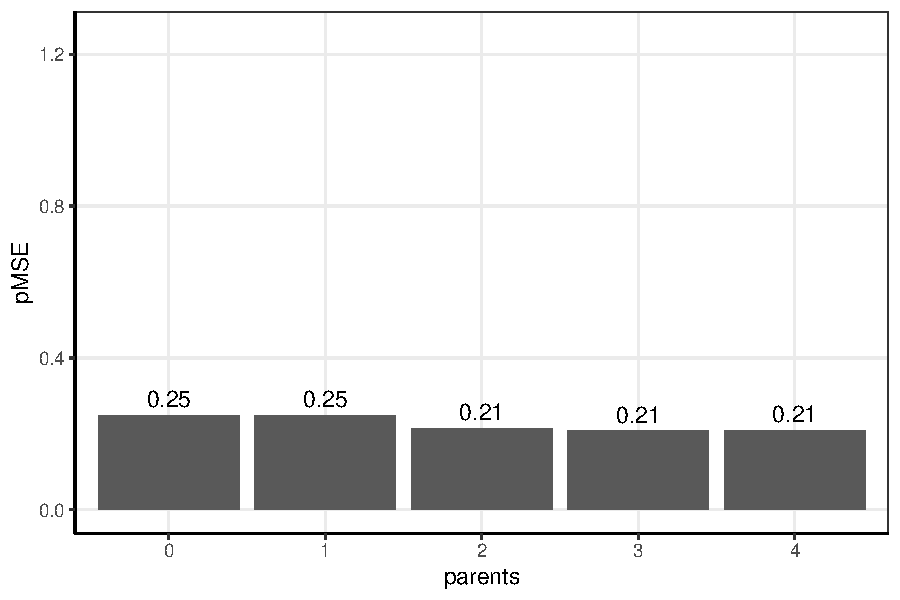
\includegraphics[width=\linewidth]{../graphs/datasynthesizer/datasynthesizer_fidelity_optimize_dataset_parents.pdf}
  \label{fig:tuning_ds_dataset}
\end{figure}

\begin{figure}[ht]
  \caption{Datasynthesizer two-way correlation  (pMSE)}
  \label{fig:ds_fidelity_two_way}
  \centering

  \begin{subfigure}{0.75\textwidth}
    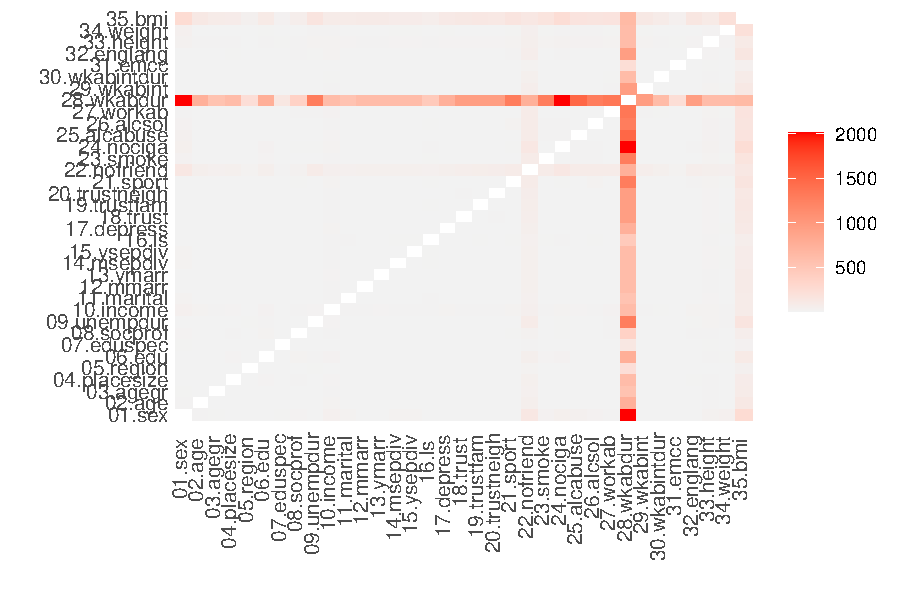
\includegraphics[width=\linewidth]{../graphs/datasynthesizer/datasynthesizer_fidelity_twoway_sd2011.pdf}
    \caption{SD2011(a)}
    \label{subfig:ds_fidelity_two_way_subfig-a}
  \end{subfigure}

  \begin{subfigure}{0.75\textwidth}
    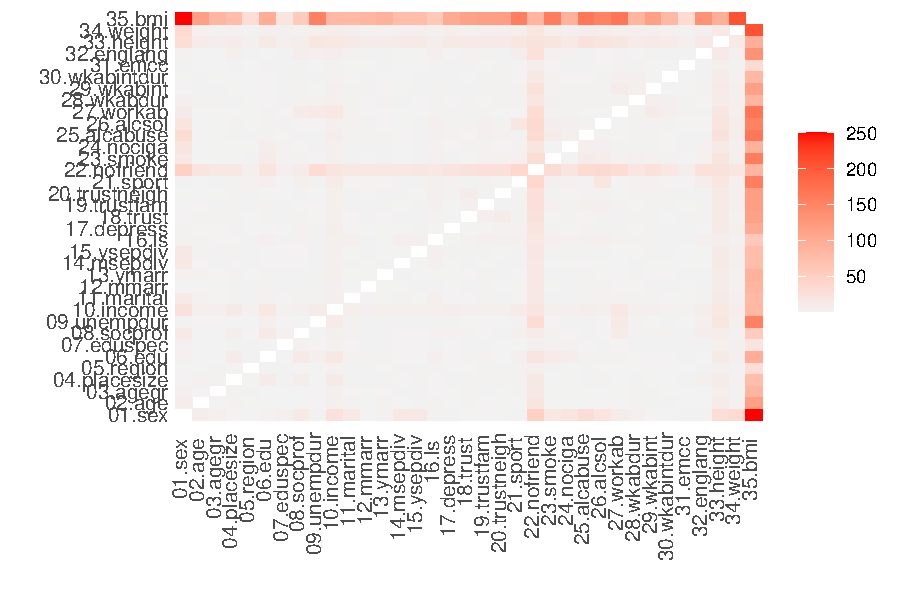
\includegraphics[width=\linewidth]{../graphs/datasynthesizer/datasynthesizer_fidelity_twoway_sd2011_clean.pdf}
    \caption{SD2011(b)}
    \label{subfig:ds_fidelity_two_way_subfig-b}
  \end{subfigure}

  \begin{subfigure}{0.75\textwidth}
    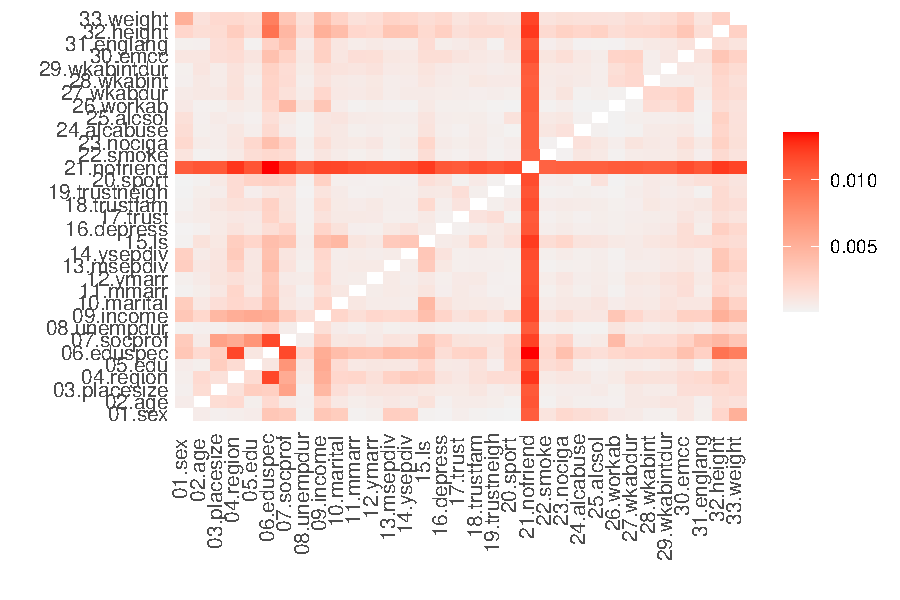
\includegraphics[width=\linewidth]{../graphs/datasynthesizer/datasynthesizer_fidelity_twoway_sd2011_clean_small.pdf}
    \caption{SD2011(c)}
    \label{subfig:ds_fidelity_two_way_subfig-c}
  \end{subfigure}
\end{figure}

\begin{figure}[ht]
  \caption{Frequency values for original and synthetic data (DataSynthesizer)}
  \label{fig:ds_variables}
  \centering

\begin{subfigure}{\textwidth}
    \caption{Variable: \texttt{wkabdur} (Work abroad duration)}
    \resizebox{\textwidth}{!}{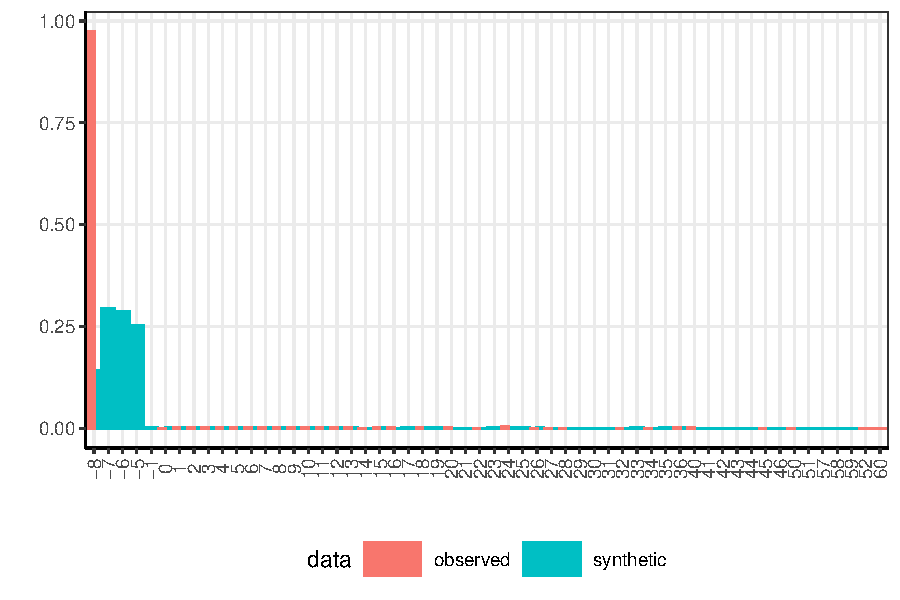
\includegraphics{../graphs/datasynthesizer/datasynthesizer_wkabdur.pdf}}
    \label{subfig:ds_variable_wkabdur}
\end{subfigure}

\begin{subfigure}{\textwidth}
    \caption{Variable: \texttt{bmi} (Body mass index)}
    \resizebox{\textwidth}{!}{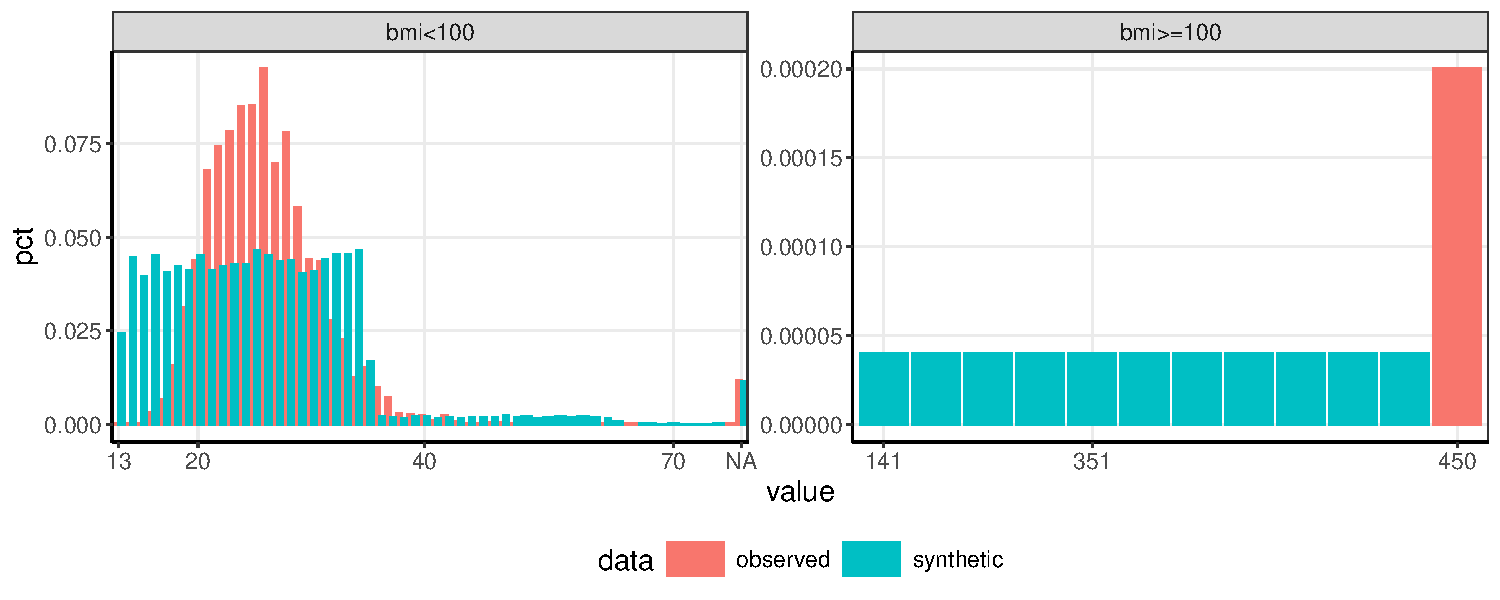
\includegraphics{../graphs/datasynthesizer/datasynthesizer_bmi.pdf}}
    \label{subfig:ds_variable_bmi}
\end{subfigure}


\begin{subfigure}{\textwidth}
    \caption{Variable: \texttt{nofriend} (Number of friends)}
    \resizebox{\textwidth}{!}{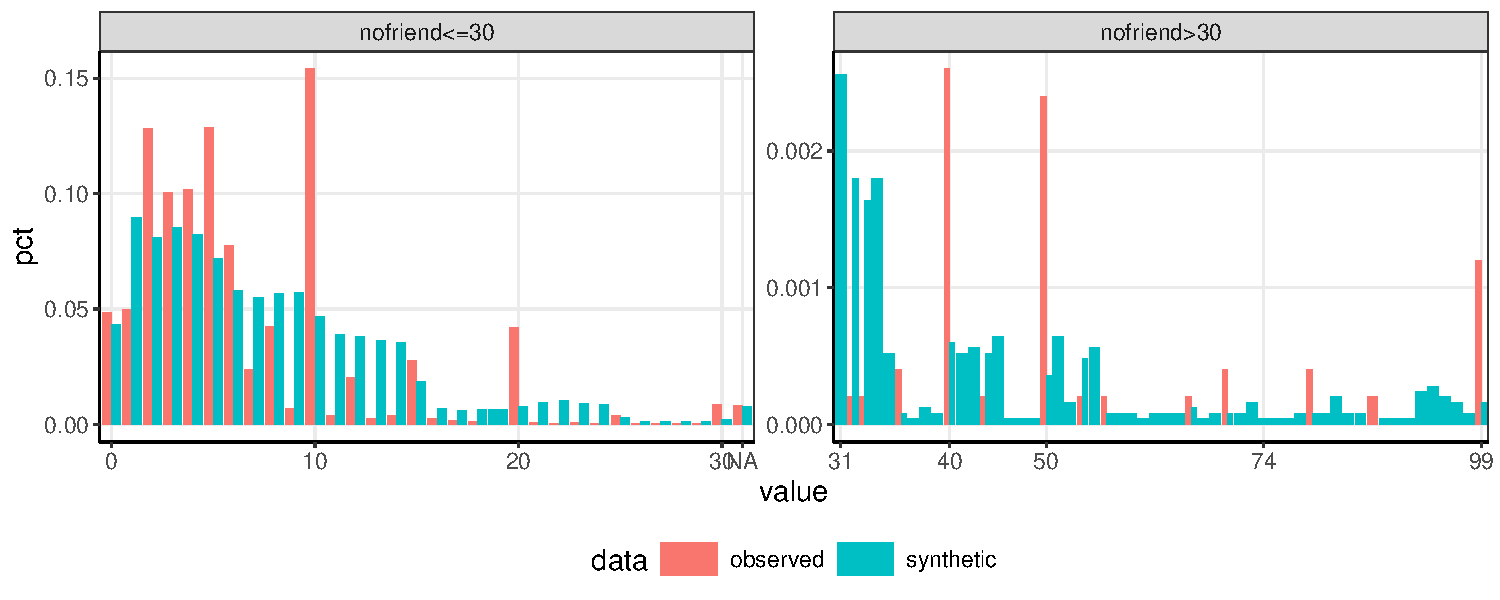
\includegraphics{../graphs/datasynthesizer/datasynthesizer_nofriend.pdf}}
    \label{subfig:ds_variable_nofriend}
\end{subfigure}
\end{figure}

\begin{figure}[ht]
  \caption{Tuning DataSynthesizer across data sets (parents = 2)}
  \label{fig:tuning_ds}
  \centering
  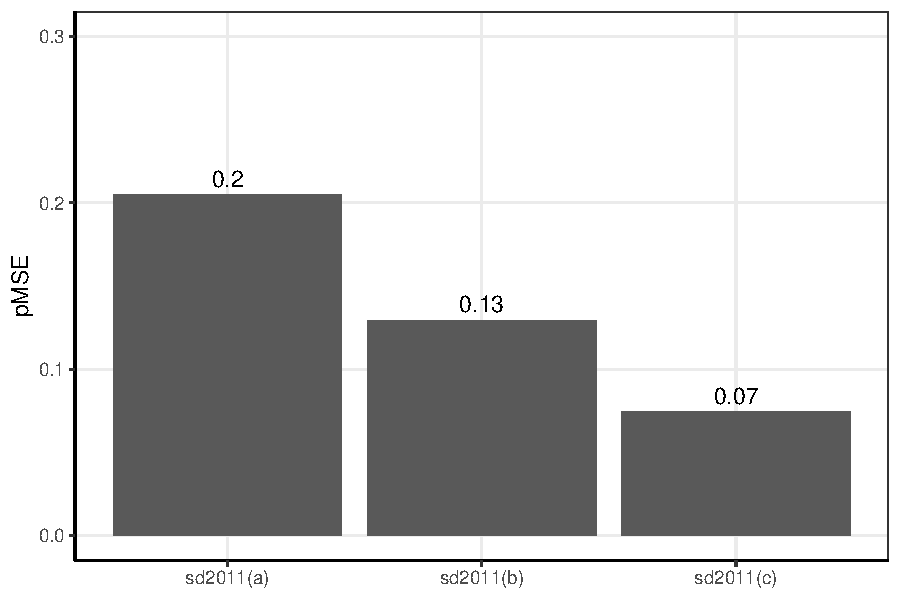
\includegraphics[width=\linewidth]{../graphs/datasynthesizer/datasynthesizer_fidelity_optimize_dataset_compare.pdf}
  \label{fig:tuning_ds_optimize_dataset_compare}
\end{figure}


%%%%%%%%%%%%%%%%%%%%%%%%%%%%%%%%%%%%%%
% Appendix
% CTGAN
%%%%%%%%%%%%%%%%%%%%%%%%%%%%%%%%%%%%%%
\clearpage
\section{Appendix: CTGAN}\label{appendix:CTGAN}
\setcounter{figure}{0}    
\setcounter{table}{0}    
\renewcommand*\thetable{\Alph{section}.\arabic{table}}
\renewcommand*\thefigure{\Alph{section}.\arabic{figure}}
\renewcommand{\theHfigure}{\Alph{section}.\arabic{table}}
\renewcommand{\theHtable}{\Alph{section}.\arabic{figure}}

\begin{table}[!h]
    \rowcolors{1}{white}{lightgray}
    \caption{Batch size and epochs = total steps}
    \centering
    \begin{tabular}{cllll>{\cellcolor{white}}p{1in}}
    % {cllllp{1in}}
    \toprule
    N & Batch size & Steps per Epoch & Epochs & Total Steps & Compare \\
    \midrule
    5.000 & 500 & 10 & 100 & 1,000 & \multirow{4}{1in}{Constant batch size, as shown in figure \ref{subfig:ctgan_fidelity_optimize_batch_size}}\\
    5.000 & 500 & 10 & 300 & 3,000 \\
    5.000 & 500 & 10 & 600 & 6,000 \\
    5.000 & 500 & 10 & 900 & 9,000 \\ \hline
    5.000 & 100 & 50 & 60 & 3,000  & \multirow{4}{1in}{Constant batch size, as shown in figure \ref{subfig:ctgan_fidelity_optimize_epochs}} \\
    5.000 & 250 & 20 & 150 & 3,000 \\
    5.000 & 500 & 10 & 300 & 3,000 \\
    5.000 & 1.000 & 5 & 600 & 3,000 \\ 
    \bottomrule
    \end{tabular}
\end{table}

\begin{figure}[ht]
  \caption{Tuning CTGAN (effect of steps)}
  \label{fig:ctgan_fidelity_optimize}
  \centering

  \begin{subfigure}{0.75\textwidth}
  \caption{Effect of batch size with constant steps (3.000)}
  \resizebox{\textwidth}{!}{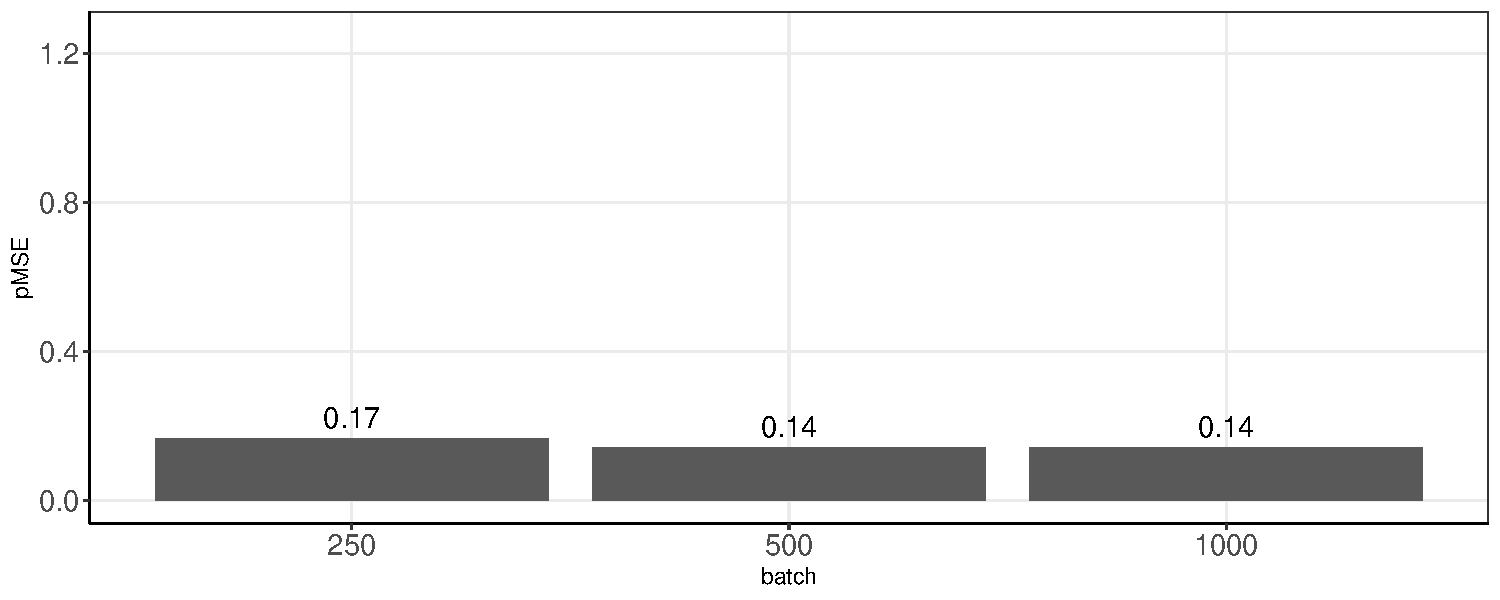
\includegraphics{../../ctgan/graphs/ctgan/ctgan_fidelity_optimize_batch_size.pdf}}
  \label{subfig:ctgan_fidelity_optimize_batch_size}
  \end{subfigure}

  \begin{subfigure}{0.75\textwidth}
  \caption{Effect of epoch number with constant batch size (500)}
  \resizebox{\textwidth}{!}{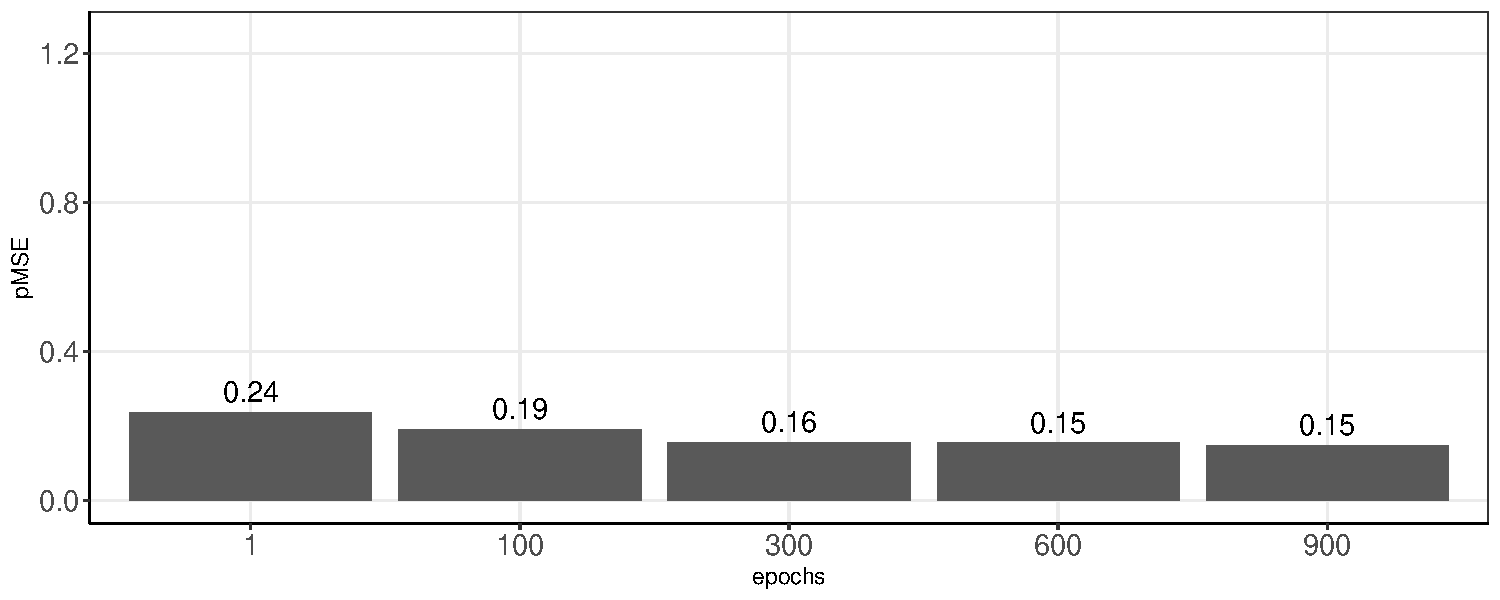
\includegraphics{../../ctgan/graphs/ctgan/ctgan_fidelity_optimize_epochs.pdf}}
  \label{subfig:ctgan_fidelity_optimize_epochs}
  \end{subfigure}

  \begin{subfigure}{0.75\textwidth}
    \caption{Effect of dimensionality}
      \resizebox{\textwidth}{!}{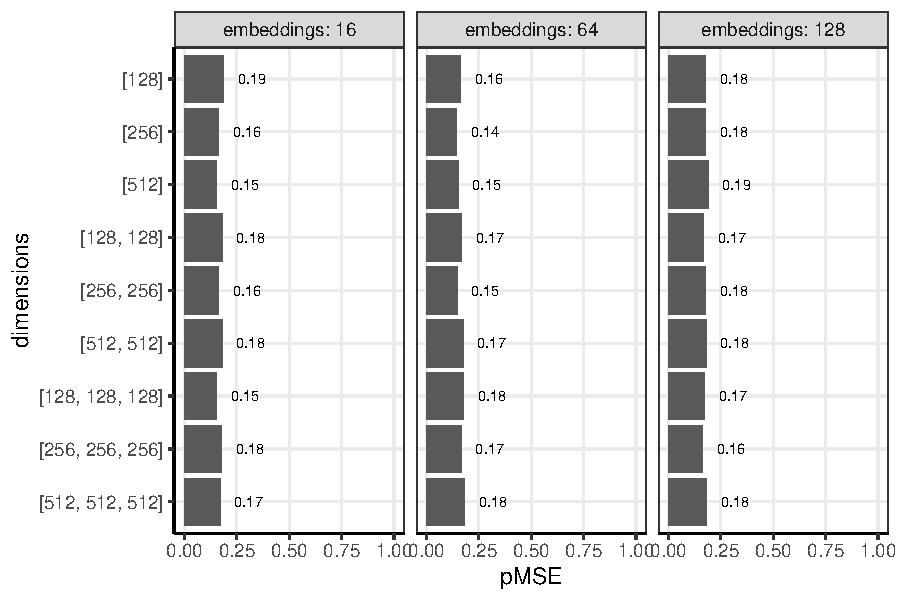
\includegraphics{../../ctgan/graphs/ctgan/ctgan_fidelity_optimize_dimensions.pdf}}
      \label{subfig:ctgan_fidelity_optimize_dimensions}
  \end{subfigure}
\end{figure}


\begin{figure}[ht]
  \caption{CTGAN two-way correlation (pMSE)}
  \label{fig:ctgan_fidelity_two_way}
  \centering

  \begin{subfigure}{0.75\textwidth}
    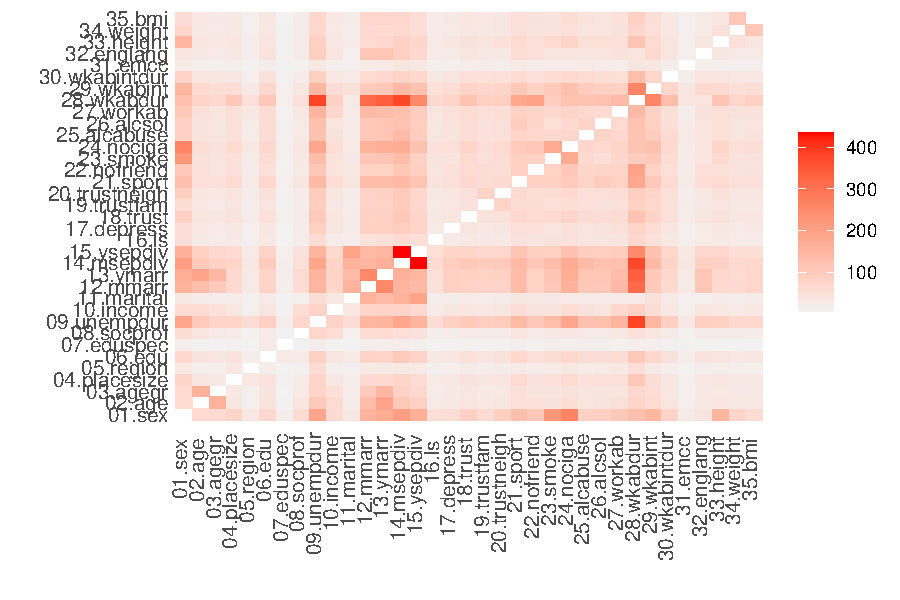
\includegraphics[width=\linewidth]{../graphs/ctgan/ctgan_fidelity_twoway_sd2011.pdf}
    \caption{SD2011(a)}
    \label{fig:ctgan_fidelity_two_way_subfig-a}
  \end{subfigure}

  \begin{subfigure}{0.75\textwidth}
    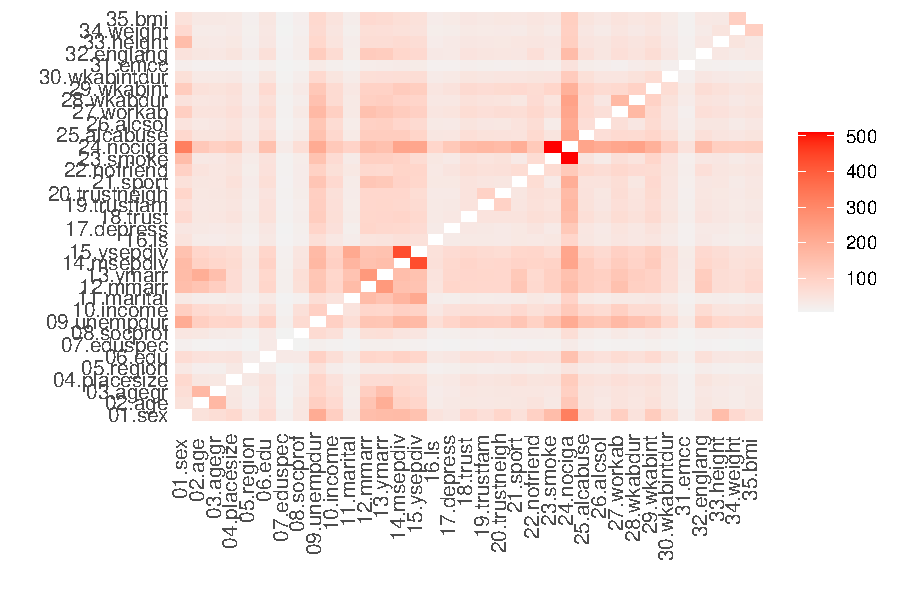
\includegraphics[width=\linewidth]{../graphs/ctgan/ctgan_fidelity_twoway_sd2011_clean.pdf}
    \caption{SD2011(b)}
    \label{fig:ctgan_fidelity_two_way_subfig-b}
  \end{subfigure}

  \begin{subfigure}{0.75\textwidth}
    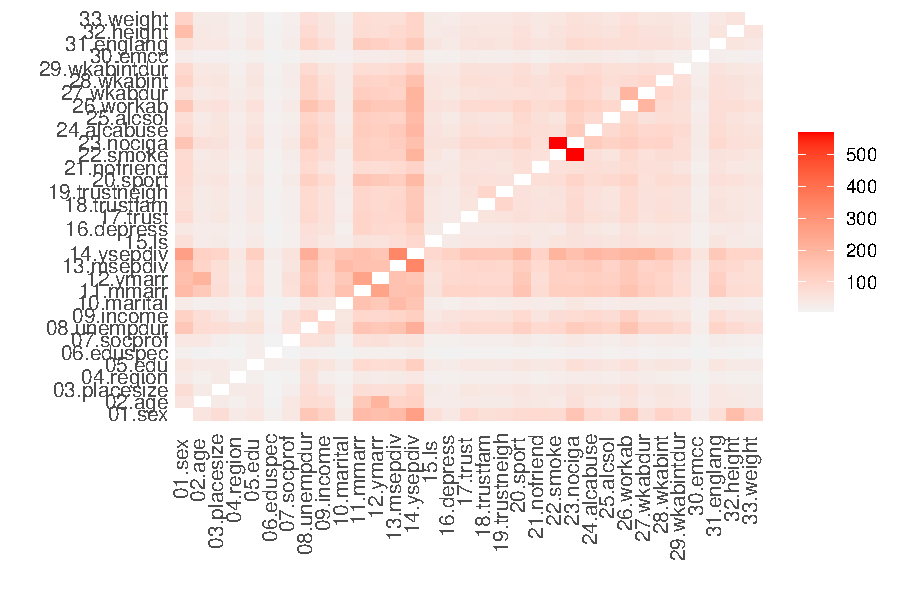
\includegraphics[width=\linewidth]{../graphs/ctgan/ctgan_fidelity_twoway_sd2011_clean_small.pdf}
    \caption{SD2011(c)}
    \label{fig:ctgan_fidelity_two_way_subfig-c}
  \end{subfigure}

\end{figure}

%%%%%%%%%%%%%%%%%%%%%%%%%%%%%%%%%%%%%%
%%%%%%%%%%%%%%%%%%%%%%%%%%%%%%%%%%%%%%
%SYNTHPOP
%%%%%%%%%%%%%%%%%%%%%%%%%%%%%%%%%%%%%%
%%%%%%%%%%%%%%%%%%%%%%%%%%%%%%%%%%%%%%
\begin{figure}[ht]
  \caption{Synthpop two-way correlation  (pMSE)}
  \label{fig:synthpop_fidelity_two_way}
  \centering

  \begin{subfigure}{0.75\textwidth}
    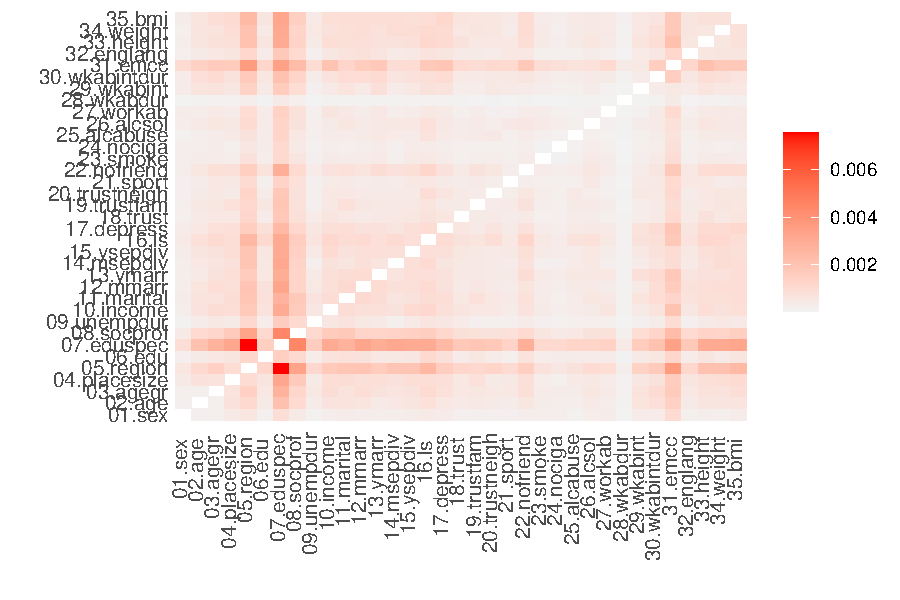
\includegraphics[width=\linewidth]{../graphs/synthpop/synthpop_fidelity_twoway_sd2011.pdf}
    \caption{SD2011(a)}
    \label{fig:synthpop_fidelity_two_way_subfig-a}
  \end{subfigure}

  \begin{subfigure}{0.75\textwidth}
    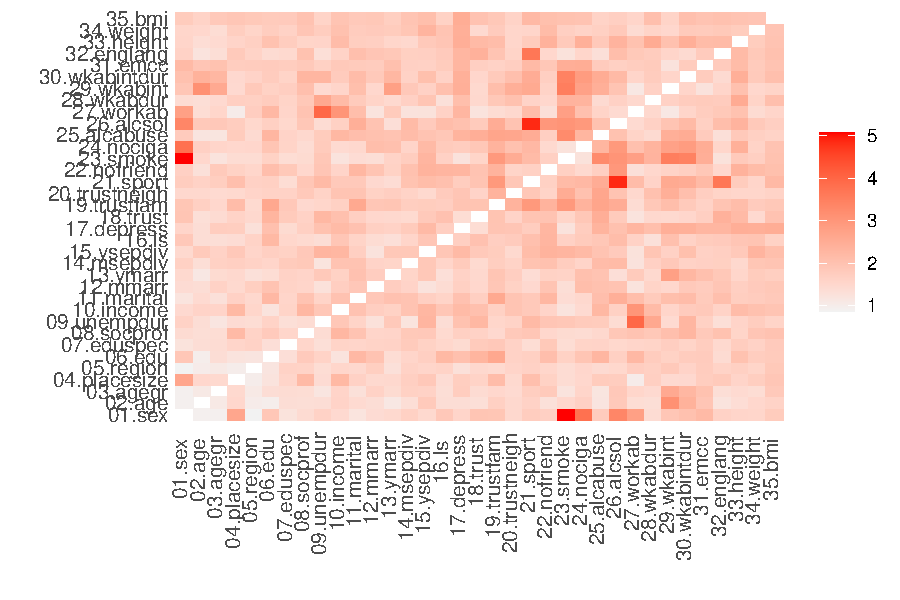
\includegraphics[width=\linewidth]{../graphs/synthpop/synthpop_fidelity_twoway_sd2011_clean.pdf}
    \caption{SD2011(b)}
    \label{fig:synthpop_fidelity_two_way_subfig-b}
  \end{subfigure}

  \begin{subfigure}{0.75\textwidth}
    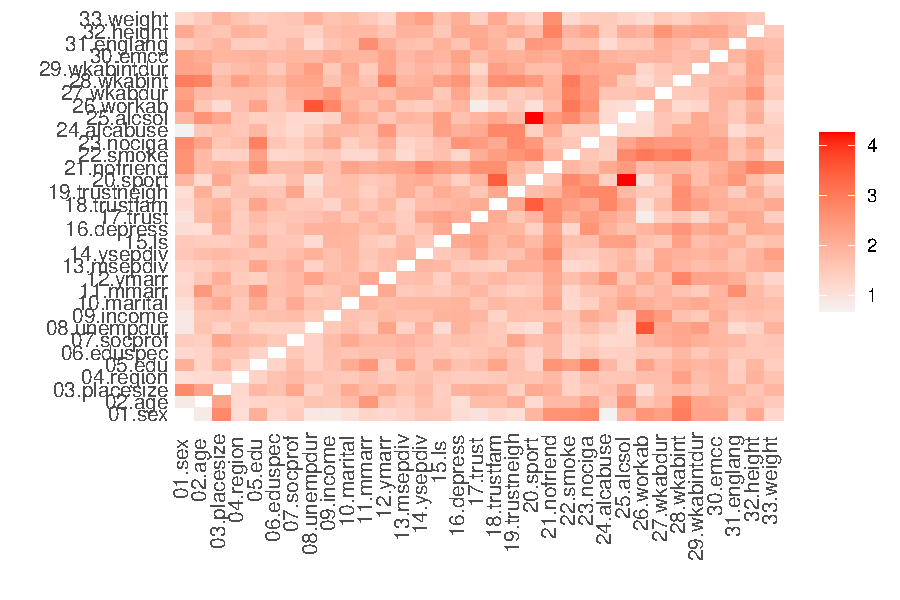
\includegraphics[width=\linewidth]{../graphs/synthpop/synthpop_fidelity_twoway_sd2011_clean_small.pdf}
    \caption{SD2011(c)}
    \label{fig:synthpop_fidelity_two_way_subfig-c}
  \end{subfigure}

\end{figure}



\end{document}
